\section{Teorema de Sharkovsky}

Nessa seção, consideraremos $f: \RR \to \RR$ uma função contínua.
Além disso, escreveremos $I_0 \longrightarrow I_1 \longrightarrow \cdots \longrightarrow I_n$ quando $I_0, \, I_1, \, \dots, \, I_n$ são intervalos compactos e $f(I_k) \supset I_{k+1}$ para todo $0 \leq k < n$.

\begin{proposition}\label{prop 9-1}
Se $I_0 \longrightarrow I_1$, então existe um intervalo fechado $I_0' \subset I_0$ tal que $f(I_0') = I_1$.
\end{proposition}

\begin{proof}
Se $I_0 = [a, b]$ e $I_1 = [c, d]$, sejam $p, \, q \in [a, b]$ tais que $f(p) = c$ e $f(q) = d$.
Suponha que $p \leq q$; se $q \leq p$, a demostração é análoga.

Definindo $b' = \inf \lbrace x \in [p, q] : f(x) = d \rbrace$ e $a' = \sup \lbrace x \in [p, b'] : f(x) = c \rbrace$ e observando que $f$ é contínua, podemos concluir que $f(I_0') = I_1$, onde $I_0' = [a', b']$.
\end{proof}

\begin{lemma}
Se $I_0 \longrightarrow I_1 \longrightarrow \cdots \longrightarrow I_{n-1} \longrightarrow I_0$, então existe $p \in I_0$ tal que as seguintes condições são válidas:
\begin{enumerate}
\item $f^k(p) \in I_k$ para todo $1 \leq k < n$.
\item $f^n(p) = p$.
\end{enumerate}
\end{lemma}

\begin{proof}
Pela Proposição \ref{prop 9-1}, podemos construir uma sequência de intervalos fechados $I_0', \, I_1', \, \dots, \, I_{n-1}'$ com as seguintes propriedades:
\begin{enumerate}[label=\alph*)]
\item \textit{$I_0 \supset I_0' \supset I_1' \supset \cdots \supset I_{n-1}'$.}
\item \textit{$f^k(I_{k-1}') = I_k$ para todo $1 \leq k < n$.}
\item \textit{$f^n(I_{n-1}') = I_0$.}
\end{enumerate}

Desse modo, existe $p \in I_{n-1}'$ tal que $f^n(p) = p$.
Em particular, $p \in I_0$ e $f^k(p) \in I_k$ para todo $1 \leq k < n$.
\end{proof}

\begin{theorem}\label{teo 9-2}
Se $\per_3(f) \neq \emptyset$, então $\per_n(f) \neq \emptyset$ para todo $n \geq 1$.
\end{theorem}

\begin{proof}
Sejam $p_1 < p_2 < p_3$ os pontos da órbita de um elemento de $\per_3(f)$. Suponha que $f(p_1) = p_2$ e $f(p_2) = p_3$; se $f(p_1) = p_3$ e $f(p_3) = p_2$, a demonstração é análoga.
Definindo $I_0 = [p_1, p_2]$ e $I_1 = [p_2, p_3]$, temos que $I_0 \longrightarrow I_1$, $I_1 \longrightarrow I_0$ e $I_1 \longrightarrow I_1$. Desse modo, podemos demonstrar as seguintes afirmações:

\begin{enumerate}[label=\alph*)]
\item \textit{$\per_1(f) \neq \emptyset$.}

De fato, $I_1 \longrightarrow I_1$ implica que existe $p \in I_1$ tal que $f(p) = p$.

\item \textit{$\per_2(f) \neq \emptyset$.}

De fato, $I_0 \longrightarrow I_1 \longrightarrow I_0$ implica que existe $p \in I_0$ tal que $f(p) \in I_1$ e $f^2(p) = p$.
Se $f(p) = p$, então $p \in I_0 \cap I_1$, o que é um absurdo pois $I_0 \cap I_1 = \lbrace p_2 \rbrace$ e $p_2 \in \per_3(f)$.

\item \textit{$\per_4(f) \neq \emptyset$.}

De fato, $I_1 \longrightarrow I_1 \longrightarrow I_1 \longrightarrow I_0 \longrightarrow I_1$ implica que existe $p \in I_1$ tal que $f^k(p) \in I_1$ para todo $1 \leq k < 3$, $f^3(p) \in I_0$ e $f^4(p) = p$.
Se $f^3(p) = p$, então $p \in I_0 \cap I_1$, o que é um absurdo pois $I_0 \cap I_1 = \lbrace p_2 \rbrace$ e $f^2(p_2) = p_1 \notin I_1$.
Se $f^k(p) = p$ para algum $1 \leq k < 3$, então $f^k(p) \in I_1$ para todo $k \geq 1$.
Em particular, $f^3(p) \in I_0 \cap I_1 = \lbrace p_2 \rbrace$ e, portanto, $f^4(p) = p = p_3$, o que é um absurdo pois $f(p_3) = p_1 \notin I_1$.
\end{enumerate}

Por fim, podemos demonstrar de maneira análoga à última afirmação que $\per_n(f) \neq \emptyset$ para todo $n \geq 4$.
\end{proof}

O Teorema \ref{teo 9-2} é um caso especial do Teorema de Sharkovsky que será enunciado na sequência.
Inicialmente, considere a seguinte ordenação dos números naturais:

\begin{definition}[Ordenação de Sharkovsky]
$$3 \, \triangleright \, 5 
\, \triangleright \, \cdots \, \triangleright \,
2 \cdot 3 \, \triangleright \, 2 \cdot 5 
\, \triangleright \, \cdots \, \triangleright \,
2^2 \cdot 3 \, \triangleright \, 2^2 \cdot 5
\, \triangleright \, \cdots \, \triangleright \,
2^k \cdot 3 \, \triangleright \, 2^k \cdot 5
\, \triangleright \, \cdots \, \triangleright \,
2^2 \, \triangleright \, 2 \, \triangleright \, 1.$$
\end{definition}

A ordenação de Sharkovsky lista todos os ímpares diferentes de $1$; depois, todos os ímpares diferentes de $1$ multiplicados por 2; depois, todos os ímpares diferentes de $1$ multiplicados por 4; e assim sucessivamente. Por fim, lista todas as potências de $2$ em ordem decrescente.

Desse modo, podemos enunciar o Teorema de Sharkovsky cuja demostração, apesar de não usar nenhuma ferramenta além daquelas usadas para demonstrar o Teorema \ref{teo 9-2}, é consideravelmente maior.

\begin{theorem}[Sharkovsky]
Se $\per_n(f) \neq \emptyset$, então $\per_m(f) \neq \emptyset$ para todo $n \, \triangleright \, m$.
\end{theorem}

\begin{proof}
Ver \cite{burns}.
\end{proof}

O Teorema de Sharkovsky pode ser usado para provar que órbitas periódicas de certos tamanhos não existem. Por exemplo, observando os gráficos de $h$, $h^2$ e $h^4$ para $\mu = 3.2$ vemos que $\per_4(h) = \emptyset$ e, portanto, $\per_n(h) = \emptyset$ para todo $n \geq 3$. Ver Figura \ref{h_3,2}.

\begin{figure}[!htb]
\centering
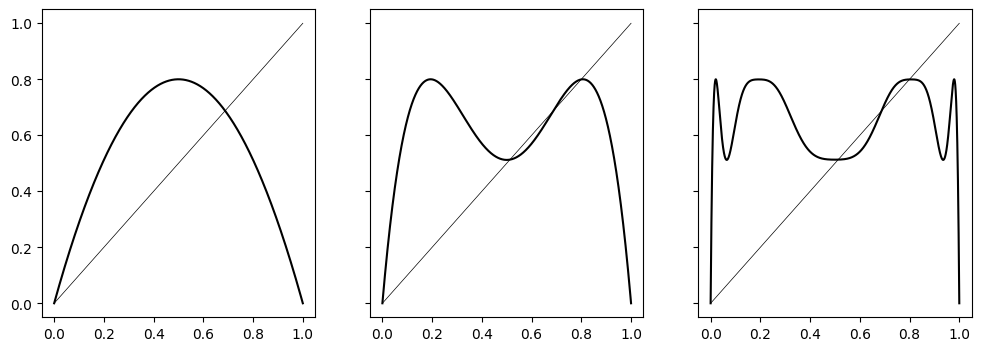
\includegraphics[scale=0.6]{images/h_3,2.png}
\caption{Gráficos de $h$, $h^2$ e $h^4$ para $\mu = 3.2$.}
\label{h_3,2}
\end{figure}

Por fim, a ordenação de Sharkovsky é a melhor possível. Se, por exemplo, $\per_5(f) \neq \emptyset$ implicasse que $\per_3(f) \neq \emptyset$, então os números $3$ e $5$ poderiam trocar de lugar nessa ordenação. O seguinte teorema mostra que isso não é possível.

\begin{theorem}
Se $n \geq 1$, então existe uma função $f$ com as seguintes propriedades:
\begin{enumerate}
\item $\per_n(f) \neq \emptyset$.
\item $\per_m(f) =  \emptyset$ para todo $m \, \triangleright \, n$.
\end{enumerate}
\end{theorem}

\begin{proof}
Seja $T: [0,1] \to [0,1]$ a função dada por
\[ T(x) =
  \begin{cases}
    2x, & x \in \left[ 0, \frac{1}{2} \right] \\
    2 - 2x, & x \in \left[ \frac{1}{2}, 1 \right] \\
  \end{cases}
\]
e considere a família de funções $T_\lambda(x) = \min \lbrace \lambda, T(x) \rbrace$ definidas em $[0,1]$, onde o parâmetro $\lambda$ varia em $[0,1]$.

Inicialmente, observe que $T(x) \leq 1$ para todo $x \in [0,1]$ implica que que $T_1 = T$.
Além disso, $T_1$ possui $2^k$ pontos periódicos de período $k$ para todo $k \geq 1$.
Desse modo, podemos definir
$$\lambda(k) = \min \lbrace \max \lbrace \orbit : \orbit \text{ é uma órbita de tamanho } k \text{ de } T_1 \rbrace \rbrace$$
para todo $k \geq 1$.
A ideia principal da prova consiste no fato de que $\lambda(k)$ desempenha os papéis de parâmetro, máximo e ponto de uma órbita de $T_{\lambda(k)}$. As seguintes afirmações tornam esse fato preciso:

\begin{enumerate}[label=\alph*)]
\item \textit{Se $\orbit \subset [0, \lambda)$ é uma órbita de $T_\lambda$, então $\orbit$ é uma órbita de $T_1$.}

Se $p \in \orbit$, então $T_\lambda(p) \in [0, \lambda)$.
Desse modo, $T_\lambda(p) = \min \lbrace \lambda, T(p) \rbrace = T(p) = T_1(p)$.
Assim, $T_\lambda$ e $T_1$ coincidem em $\orbit$ e, portanto, $\orbit$ é uma órbita de $T_1$.

\item \textit{Se $\orbit \subset [0, \lambda]$ é uma órbita de $T_1$, então $\orbit$ é uma órbita de $T_\lambda$.}

Se $p \in \orbit$, então $T_1(p) \in [0, \lambda]$. Desse modo, $T_\lambda(p) = \min \lbrace \lambda, T_1(p) \rbrace = T_1(p)$.
Assim, $T_\lambda$ e $T_1$ coincidem em $\orbit$ e, portanto, $\orbit$ é uma órbita de $T_\lambda$.

\item \textit{$T_{\lambda(k)}$ possui uma órbita $\orbit \subset [0, \lambda(k))$ de tamanho $j$ se, e somente, se $\lambda(k) > \lambda(j)$.}

Se $T_{\lambda(k)}$ possui uma órbita $\orbit \subset [0, \lambda(k))$ de tamanho $j$, então $\orbit$ é uma órbita de $T_1$ e, pela definição de $\lambda(j)$, concluímos que $\lambda(k) > \lambda(j)$.
Por outro lado, se $\lambda(k) > \lambda(j)$, então $T_1$ possui uma órbita $\orbit \subset [0, \lambda(j)] \subset [0, \lambda(k)]$ de tamanho $j$ e, desse modo, $\orbit$ é uma órbita de $T_{\lambda(k)}$.

\item \textit{A órbita de $T_1$ que contém $\lambda(k)$ é uma órbita de tamanho $k$ de $T_{\lambda(k)}$.
Além disso, todas as outras órbitas de $T_{\lambda(k)}$ estão em $[0, \lambda(k))$.} 

Pela definição de $\lambda(k)$, $T_1$ possui uma órbita $\orbit \subset [0, \lambda(k)]$ de tamanho $k$ e, portanto, $\orbit$ é uma órbita de $T_{\lambda(k)}$.

Na segunda parte, basta observar que $\lambda(k)$ é o valor máximo de $T_{\lambda(k)}$ e, desse modo, toda órbita de $T_{\lambda(k)}$ está contida em $[0, \lambda(k)]$.
Em particular, se a órbita não contém $\lambda(k)$, então ela está contida em $[0, \lambda(k))$.

\item \textit{$k \, \triangleright \, j$ se, e somente se, $\lambda(k) > \lambda(j)$.}

Suponha que $k \, \triangleright \, j$. Sabemos que $T_{\lambda(k)}$ possui uma órbita de tamanho $k$ e, pelo Teorema de Sharkovsky, $T_{\lambda(k)}$ admite uma órbita de tamanho $j$. Em particular, essa órbita está contida em $[0, \lambda(k))$ e, portanto, $\lambda(k) > \lambda(j)$.

Suponha que $\lambda(k) > \lambda(j)$. Se $j \, \triangleright \, k$, então $\lambda(k) < \lambda(j)$ pela demonstração no parágrafo anterior e, portanto, $k \, \triangleright \, j$.
\end{enumerate}

Desse modo, $T_{\lambda(n)}$ possui órbita de tamanho $n$ para cada $n \geq 1$. Além disso, se $m \, \triangleright \, n$ então $\lambda(m) > \lambda(n)$ e, portanto, $T_{\lambda(n)}$ não possui órbita de tamanho $m$.
\end{proof}
